\chapter{OpenFOAM Detonation Modeling}
\label{solvtestchap}

\section{Preface}

This chapter will go through progression of research on efficacy for the different solvers and detonation modeling techniques performed during the duration of this thesis work. In an effort to assist the University of Colorado's Turbulence and Energy Systems Laboratory (TESLa), several solvers and methods will be tested for potential for detonation modeling, stability, and accuracy, typically in that order. Additional focus will be on the effects of AMR on the results. 

\section{Modeling Progression}
\subsection{Initial Attempts}
To begin on the problem of modeling detonations in OpenFOAM, the included tutorials folder as well as the geometric and initial condition setup of located in a related TESLa paper by Towery\cite{towery1} was utilized to begin the work towards an OpenFOAM model of a linear detonation tube/PDE.

Firstly, the detonation of methane fuel and oxygen oxidizer without inert nitrogen filler was explored within a 2D detonation tube with the solver \verb|rhoReactingFoam|. A region of high temperature methane and oxygen on the left hand side was used to initiate the detonation. In the PDE and detonation simulations presented in this paper, stoichiometric fuel and oxidizer was premixed and available thoughout the domain. Solid walls on the left, top, and bottom of the tube were used. The exit was set as a special \verb|waveTransmissive| boundary condition that allows for shockwaves to not reflect at the exit and for gases to expel as well. A detonation was successfully created with this, but the accuracy and stability were still untested. In order to check that the boundary conditions being applied were correct, a small detonation cell of high pressure and temperature was set in the bottom left corner of the tube. As the simulation progressed, correct wave reflection was seen on the sides of the tube as well as some wave transmissive behavior from the exit was seen (Figure \ref{fig:cornerdet}). 
\begin{figure}[b]
\centering
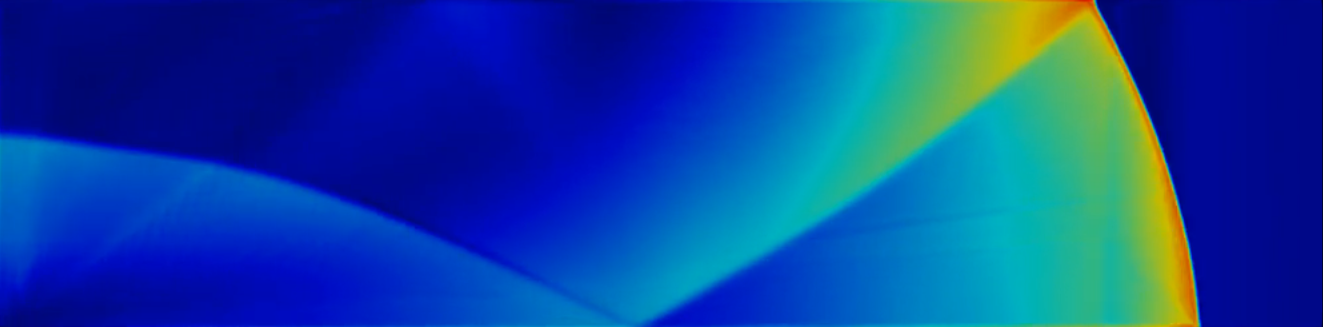
\includegraphics[width=\linewidth]{figs/cornerdet.png}
\caption{Initial methane and oxygen detonation boundary condition test with corner detonation. Velocity magnitude is plotted here without scale to just check the solver and boundary conditions for modeling potential. Detonation was initiated in the lower left corner.}
\label{fig:cornerdet}
\end{figure}%
\noindent It was noticed that the exit boundary condition was expelling gas in a rectangular region long before the detonation wave(s) reached the exit, so some tweaking was done on this \verb|waveTransmissive| boundary condition in order to make it more accurate. The boundary condition option accepts inputs such as ratio of specific heats, expected flow velocity, far-field conditions and distance from exit plane, and names of some variables such as the condition to track at the exit as well as some flux variables. 

The next step with \verb|rhoReactingFoam| was to start progressing towards testable detonation results. To do this, a change from methane to hydrogen for the fuel was selected. This fuel change was done to better match papers such as those being produced by TESLa as well as the general experimental and computational detonation modeling community. The exact geometric detontion tube was taken from Towery\cite{towery1} for comparison as well as the initial detonation size and thermodynamic conditions. Additionally, inert nitrogen was added into the tube to transition from hydrogen-oxygen to hydrogen-air. In accordance with trying to double check whether results made sense with Towery\cite{towery1}, the Arrhenius rate equation was used for reaction rates. An issue that was problematic starting this research was that the documentation for the units within the \verb|reactions| file were conflicting. Much testing was performed at this stage in an attempt to determine the units that OpenFOAM uses for the reactions given in this file, especially regarding the pre-exponential factor. While some ground was gained on this, a shift of focus towards the solver performed in order to determine if \verb|rhoReactingFoam| was appropriate for capturing shocks. 

The Sod shock tube problem was utilized to determine if the OpenFOAM solvers used were capturing shocks accurately. This problem typically consists of placing a region of higher pressure and density fluid in one region and a lower pressure and density fluid in another adjacent region. Typically the regions are rectangular and share a face, both comprising a large cube. When the simulation starts, a shock will form due to the immediate differential in pressure and density from one region to the next. This problem cannot be verified perfectly experimentally, but it can be solved analytically, making this a good method to test numerical CFD solvers for compressible flow accuracy as well as their ability to capture shocks. The results for \verb|rhoReactingFoam| matched published analytical results as well as a \verb|rhoPimpleFoam| case that was matched to the analytical results. Due to this, it was thought that \verb|rhoReactingFoam| would be a good candidate for detonation modeling. 

The next stage consisted of testing different mesh refinement levels, before AMR was utilized. The domain will be expanded on in later chapters, but the domain considered for the initial work is 0.5 meters in length and 0.04 meters square in width. Different static mesh resolutions were tested, such as 5000-1-1, 5000-3-3, 1000-80-1, 1000-3-1, and 10000-2-1. Additionally, some different time steps were tested. At this stage, it was found that there was significant noise and instability in the detonation wave solution, such that consideration of a different solver was advisable. We next tried moving towards OpenFOAM solvers utilizing central-upwind schemes of Kurganov and Tadmor, as they should perform better for detonations due to their design around compressible flow. 


\subsection{Final Solver}

The final solver settled on for this research was \verb|rhoReactingCentralFoam|. This is a solver combined together by Caelan Lapoint and the testing and validation of it is part of this thesis work. First, \verb|rhoReactingCentralFoam| was tested to see if it was accurately capturing shocks like its sister solver, \verb|rhoCentralFoam|. OpenFOAM includes a validated shock tube case utilizing \verb|rhoCentralFoam|, so the results of this were compared to \verb|rhoReactingCentralFoam|'s results in Figure \ref{fig:sod}. 
\begin{figure}
\centering
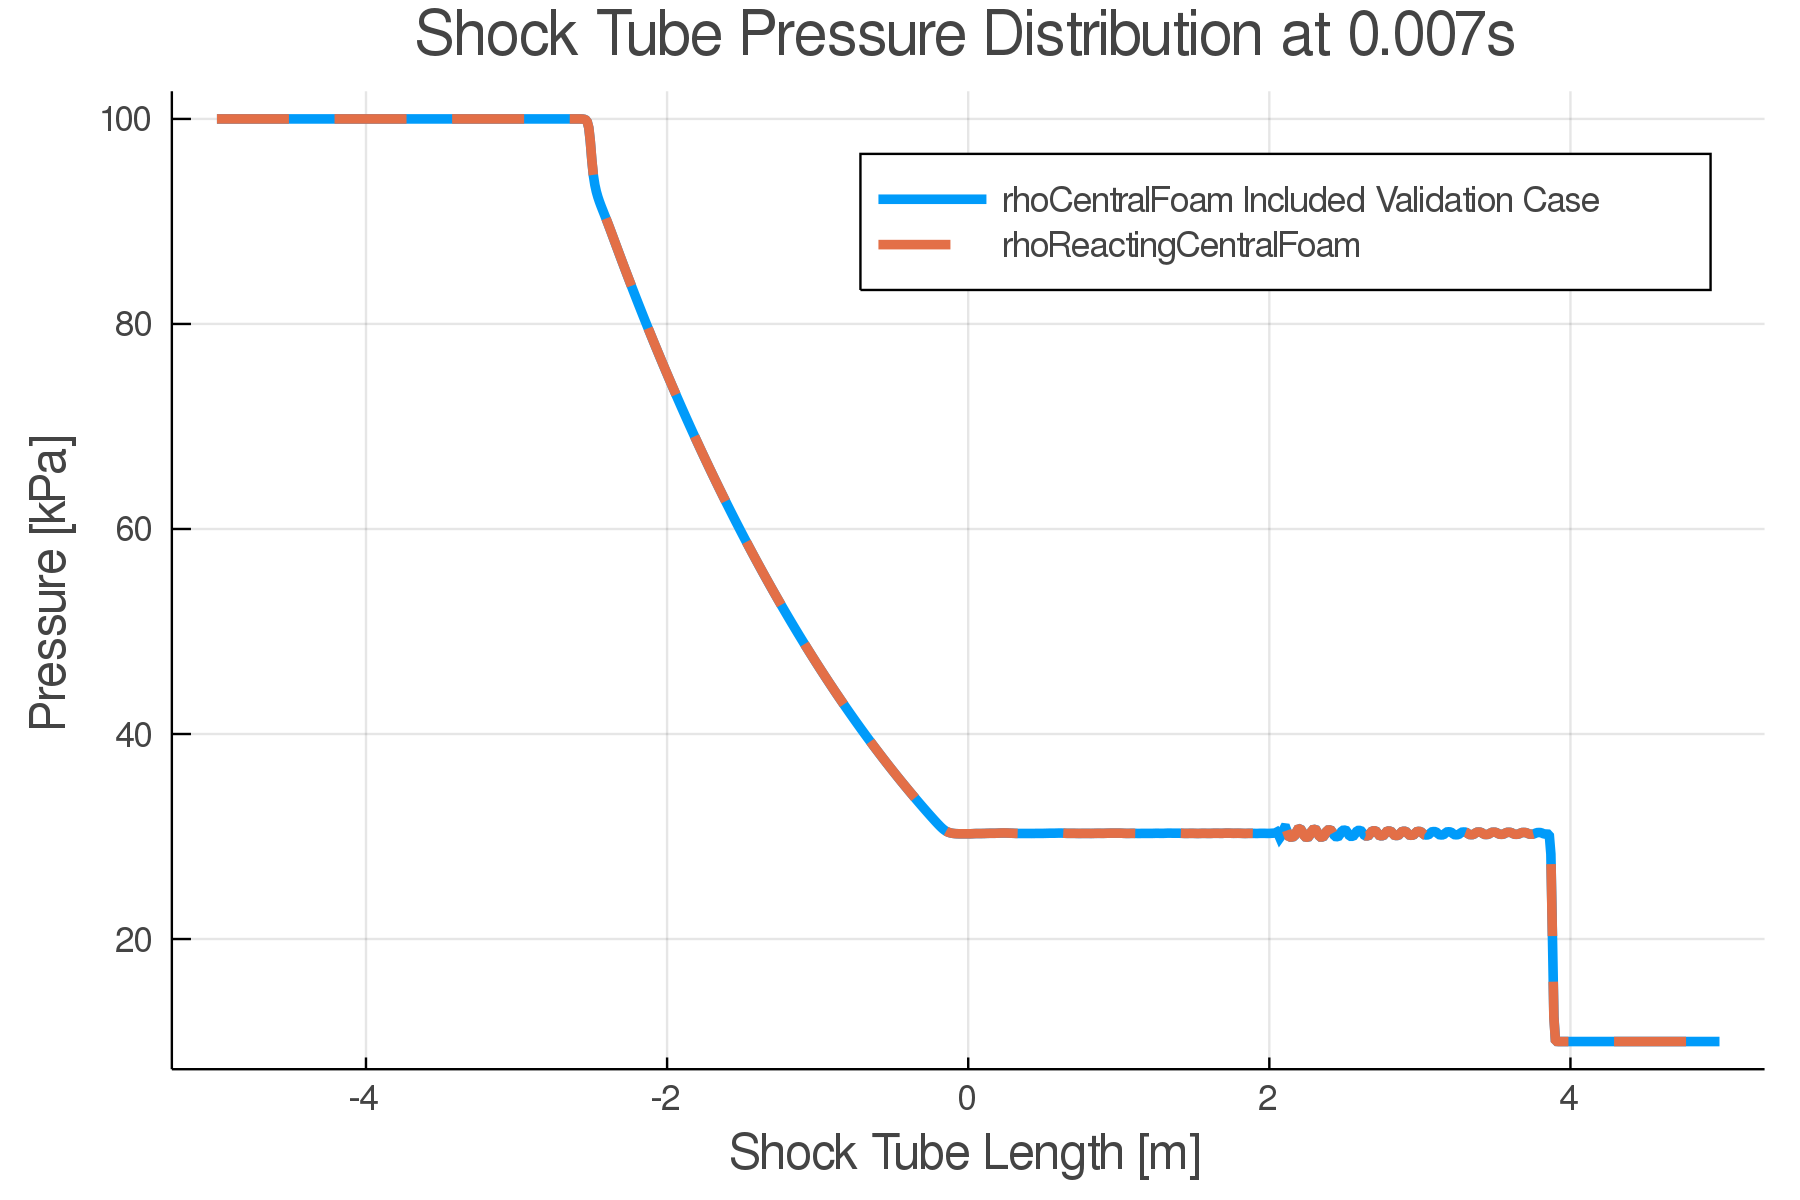
\includegraphics[width=0.85\linewidth]{./figs/shocktube.png} 
\caption{Shock tube validated test case included with OpenFOAM compared to hybrid solver}
\label{fig:sod}
\end{figure}%
\noindent It can be seen that the validation case and \verb|rhoReactingCentralFoam| match precisely, and this was expected. 


\section{Solver Parameter Testing and Sensitivity}
Line plots seen in the upcoming sections were sampled with the OpenFOAM utility \verb|postProcess|, using 1000 sampling points. The line progresses from the edge of the initiation of the detonation to the end of the detonation tube. 


\subsection{Arrhenius Pre-exponential Factor}
Now that an appropriate solver was selected, the solver settings needed to be dialed in. To start, some further testing was performed on the units of the pre-exponential factor for the Arrhenius equation in the \verb|reactions| file. Since the geometry, boundary, and initial conditions are all matched to the setup for the detonation tube in Towery\cite{towery1}, we will use the results there as a generic target to determine the order of magnitude of the exponent on the pre-exponential factor. The exponent was swept between \(10^{11}\) through \(10^{17}\). The results are seen in Figures \ref{fig:atestp}, \ref{fig:atestt}, and \ref{fig:atestu}. 

\begin{figure}
\centering
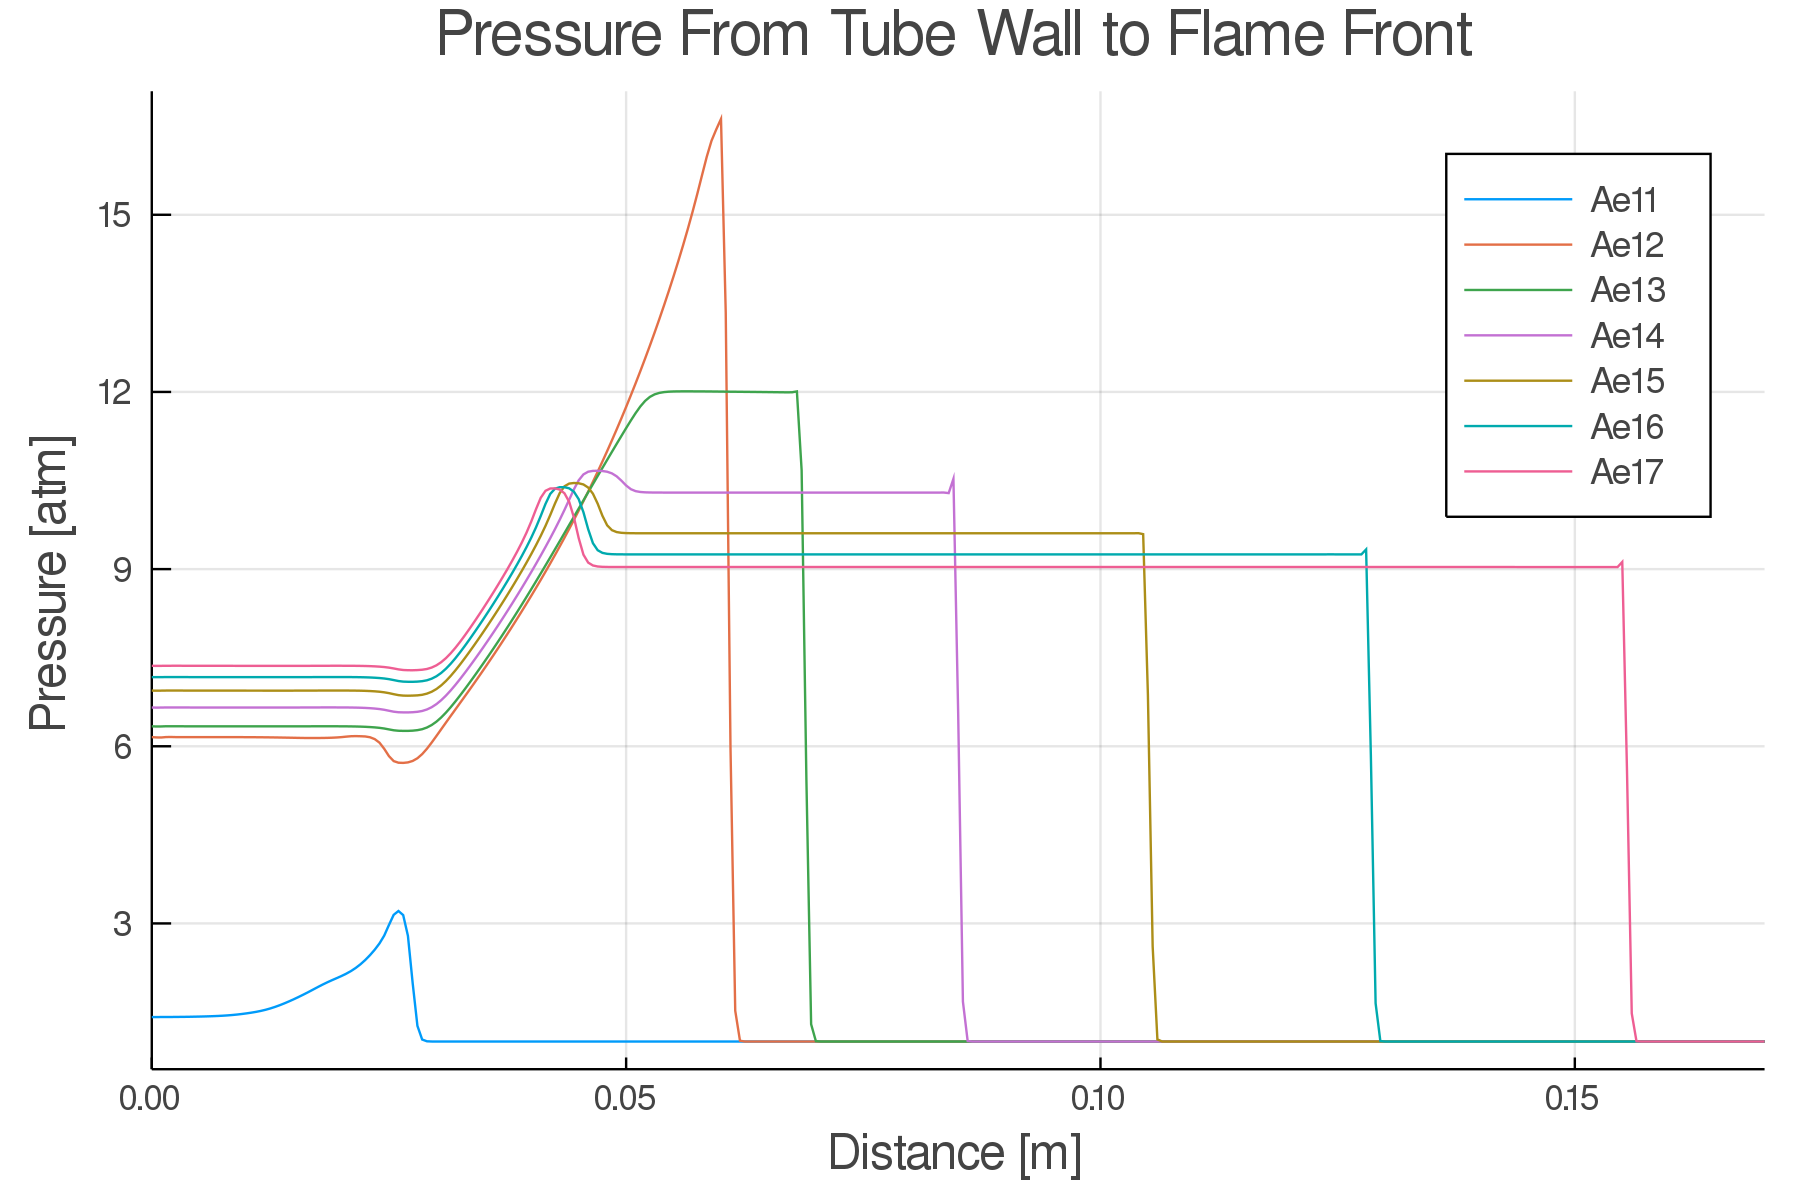
\includegraphics[width=0.85\linewidth]{./figs/Atest/p.png}
\caption{Pressure distribution in detonation tube for pre-exponential factor exponent sweep test}
\label{fig:atestp}
\end{figure}

\begin{figure}
\centering
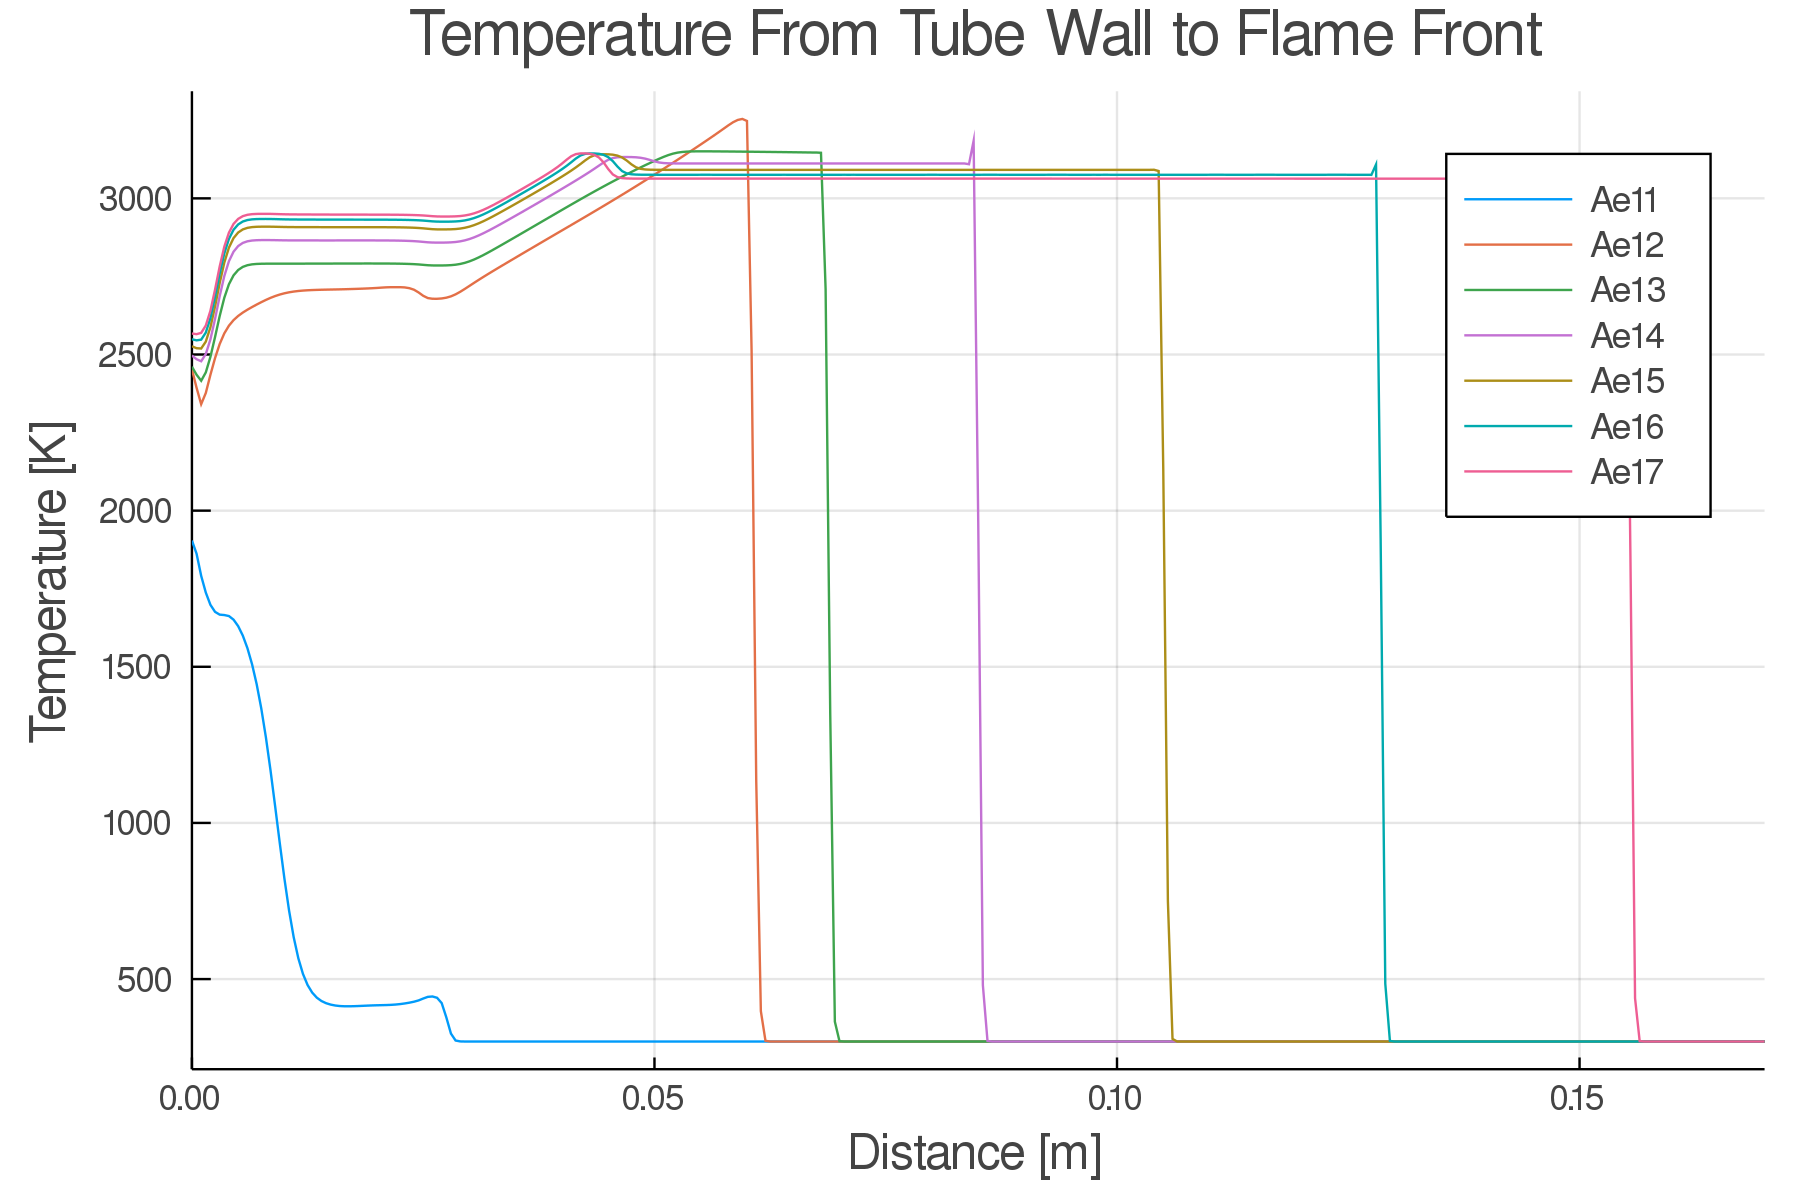
\includegraphics[width=0.85\linewidth]{./figs/Atest/t.png}
\caption{Temperature distribution in detonation tube for pre-exponential factor exponent sweep test}
\label{fig:atestt}
\end{figure}

\begin{figure}
\centering
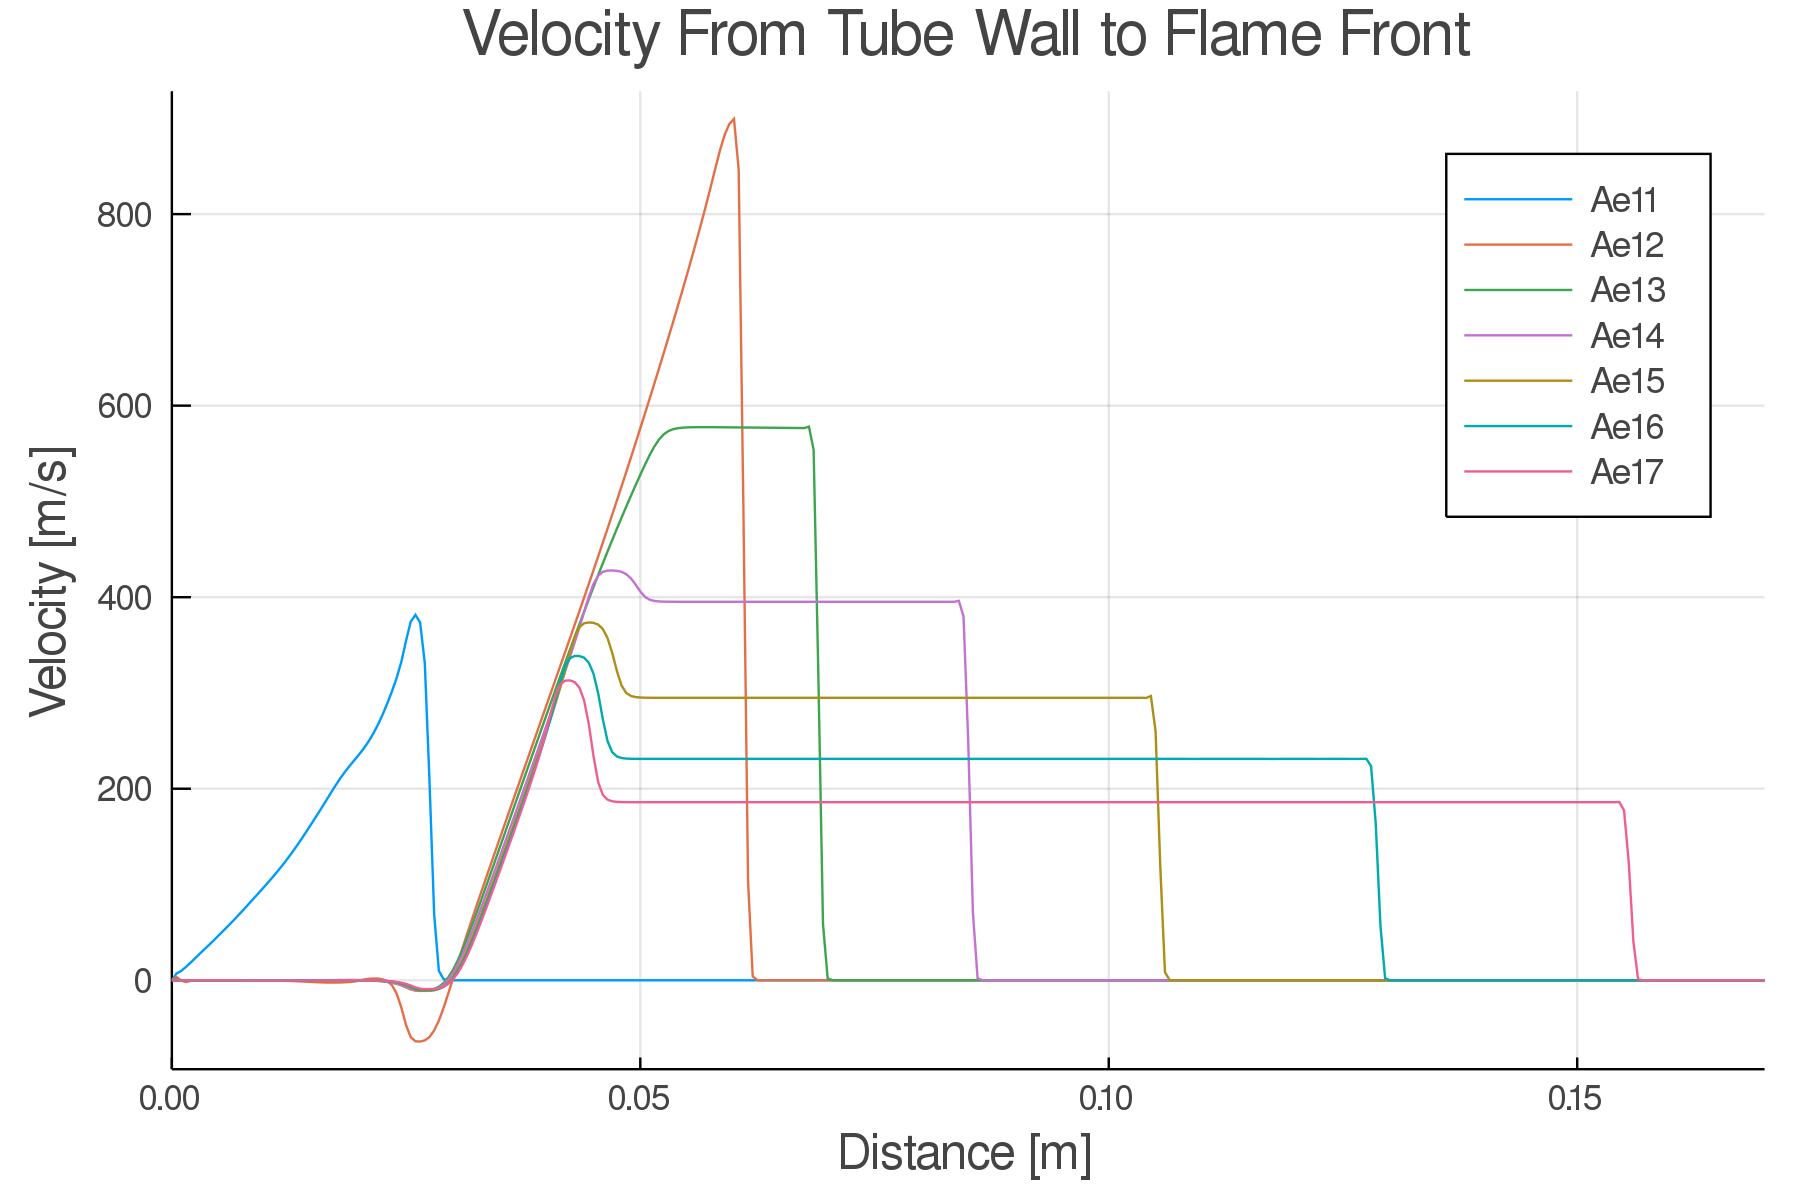
\includegraphics[width=0.85\linewidth]{./figs/Atest/u.png}
\caption{Velocity distribution in detonation tube for pre-exponential factor exponent sweep test}
\label{fig:atestu}
\end{figure}

From these figures, we can see the importance of having an accurate order of magnitude on the exponent for results. As the exponent was increased beyond the power of 12, plateaus emerge in the results for all thermodynamic variables. Under the power of 12, there is a large jump in solution, and a transition from between detonation states, seen in Figure \ref{fig:pjump}. The differences in these states is due to the coupling of the shockwave and the reactions. The grouping of plots with higher pressure values have the reactions coupled with the shock, and the smaller pressure value grouping has the reaction occurring more slowly and trailing behind the shock. This is more evident in Figures \ref{fig:atestrp} and \ref{fig:atestrt} where we see that there is still a shockwave present in the ``lower'' group, but it is clear by Figure \ref{fig:atestrt} that the reaction process is happening much later than the shockwave instead right at the shock front. Thus presence of a shockwave in this scenario is not due to the sustained reaction, and was triggered by high pressure (and temperature) region used to initialize detonations in the simulation. 

\begin{figure}
\centering
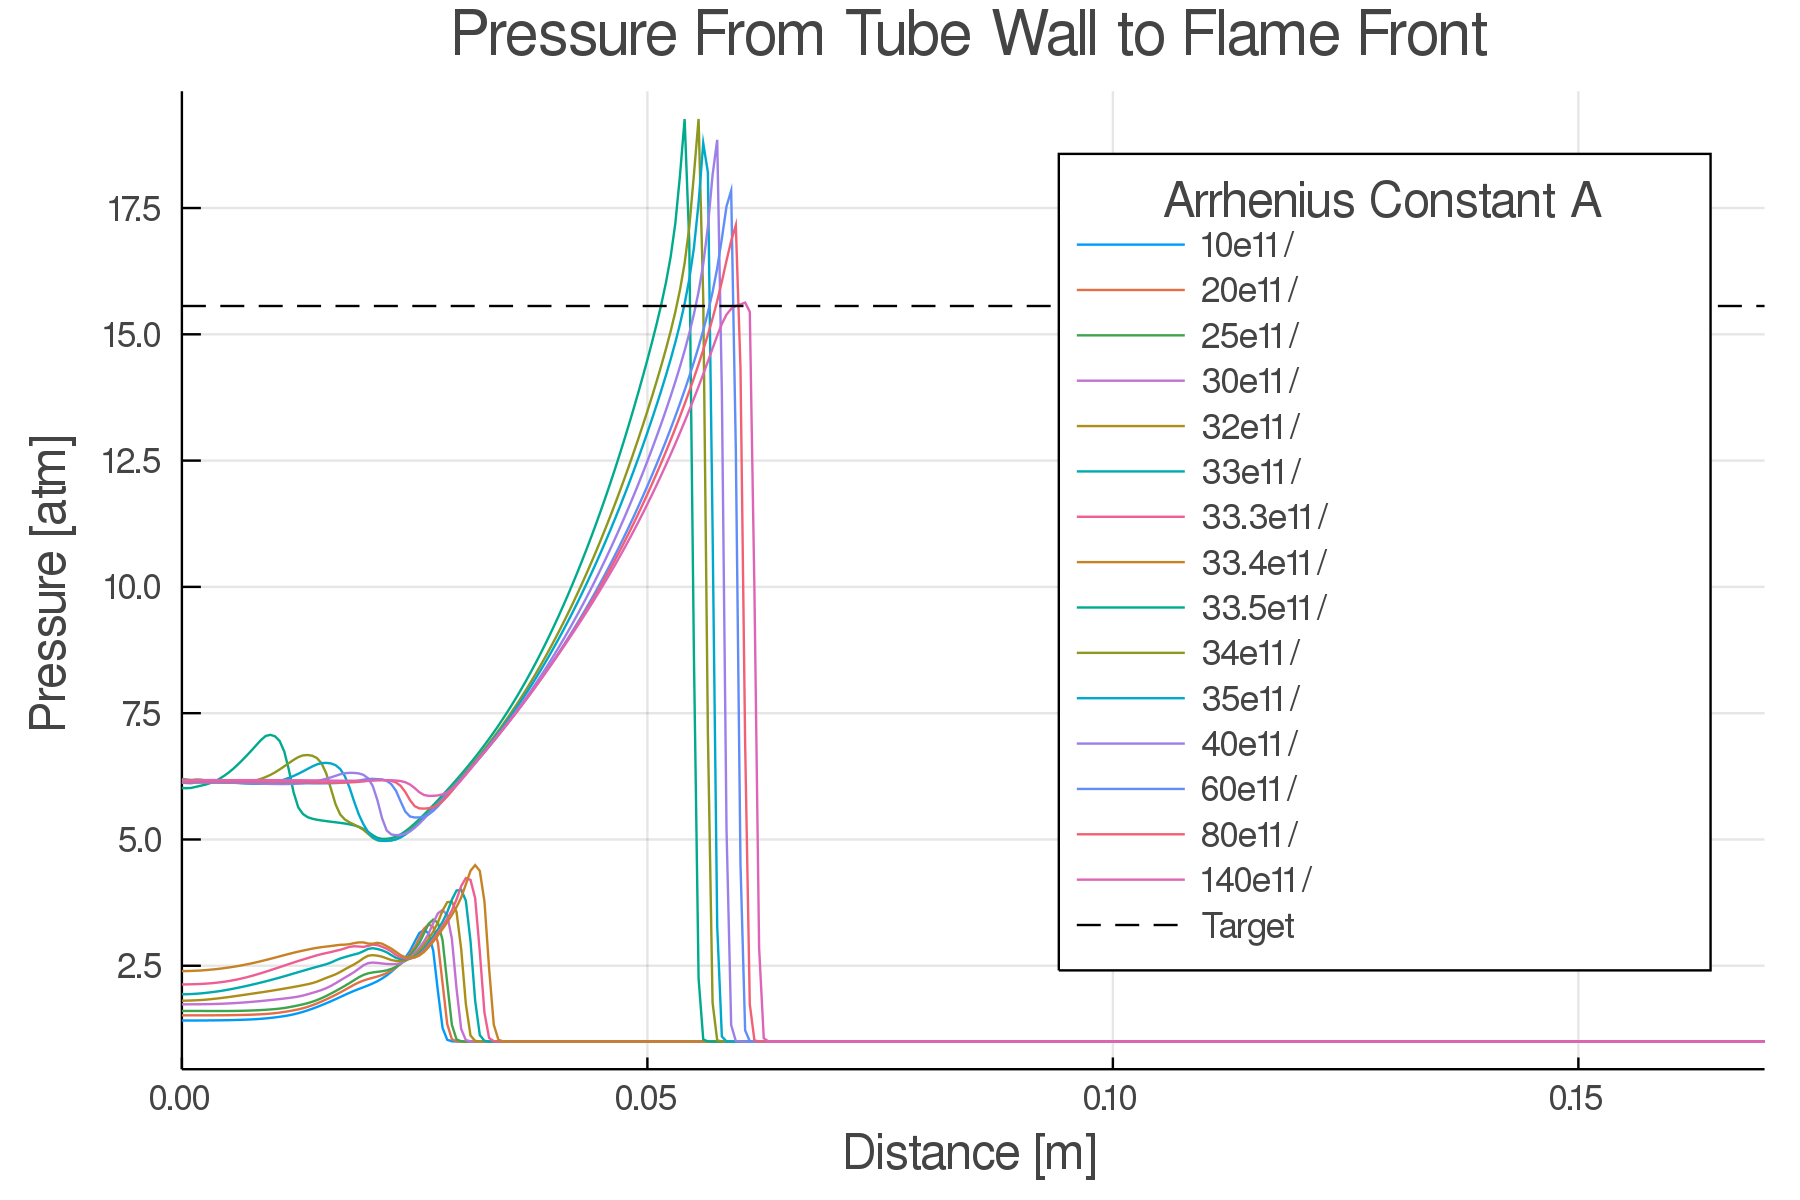
\includegraphics[width=0.85\linewidth]{./figs/Atest_refined/p_large.png}
\caption{Pressure distribution in detonation tube for expanded and refined pre-exponential factor exponent sweep test, showing detonation shock-reaction coupling transition. See Figures \ref{fig:atestrp} and r\ref{fig:atestrt} for a filtered version.}
\label{fig:pjump}
\end{figure}


The exponent in this region was explored further since plateaus in thermodynamic properties values are not physical for real-world detonations. Note that the velocity plotted in Figure \ref{fig:atestu} is a fluid velocity, not a wave velocity. When instead we swept over a smaller interval, with the Chapman-Jouguet (CJ) targets from Towery\cite{towery1} plotted, we can see that there is a very abrupt transition in detonation stability (Figures \ref{fig:atestrp} and \ref{fig:atestrt}). 

\begin{figure}
\centering
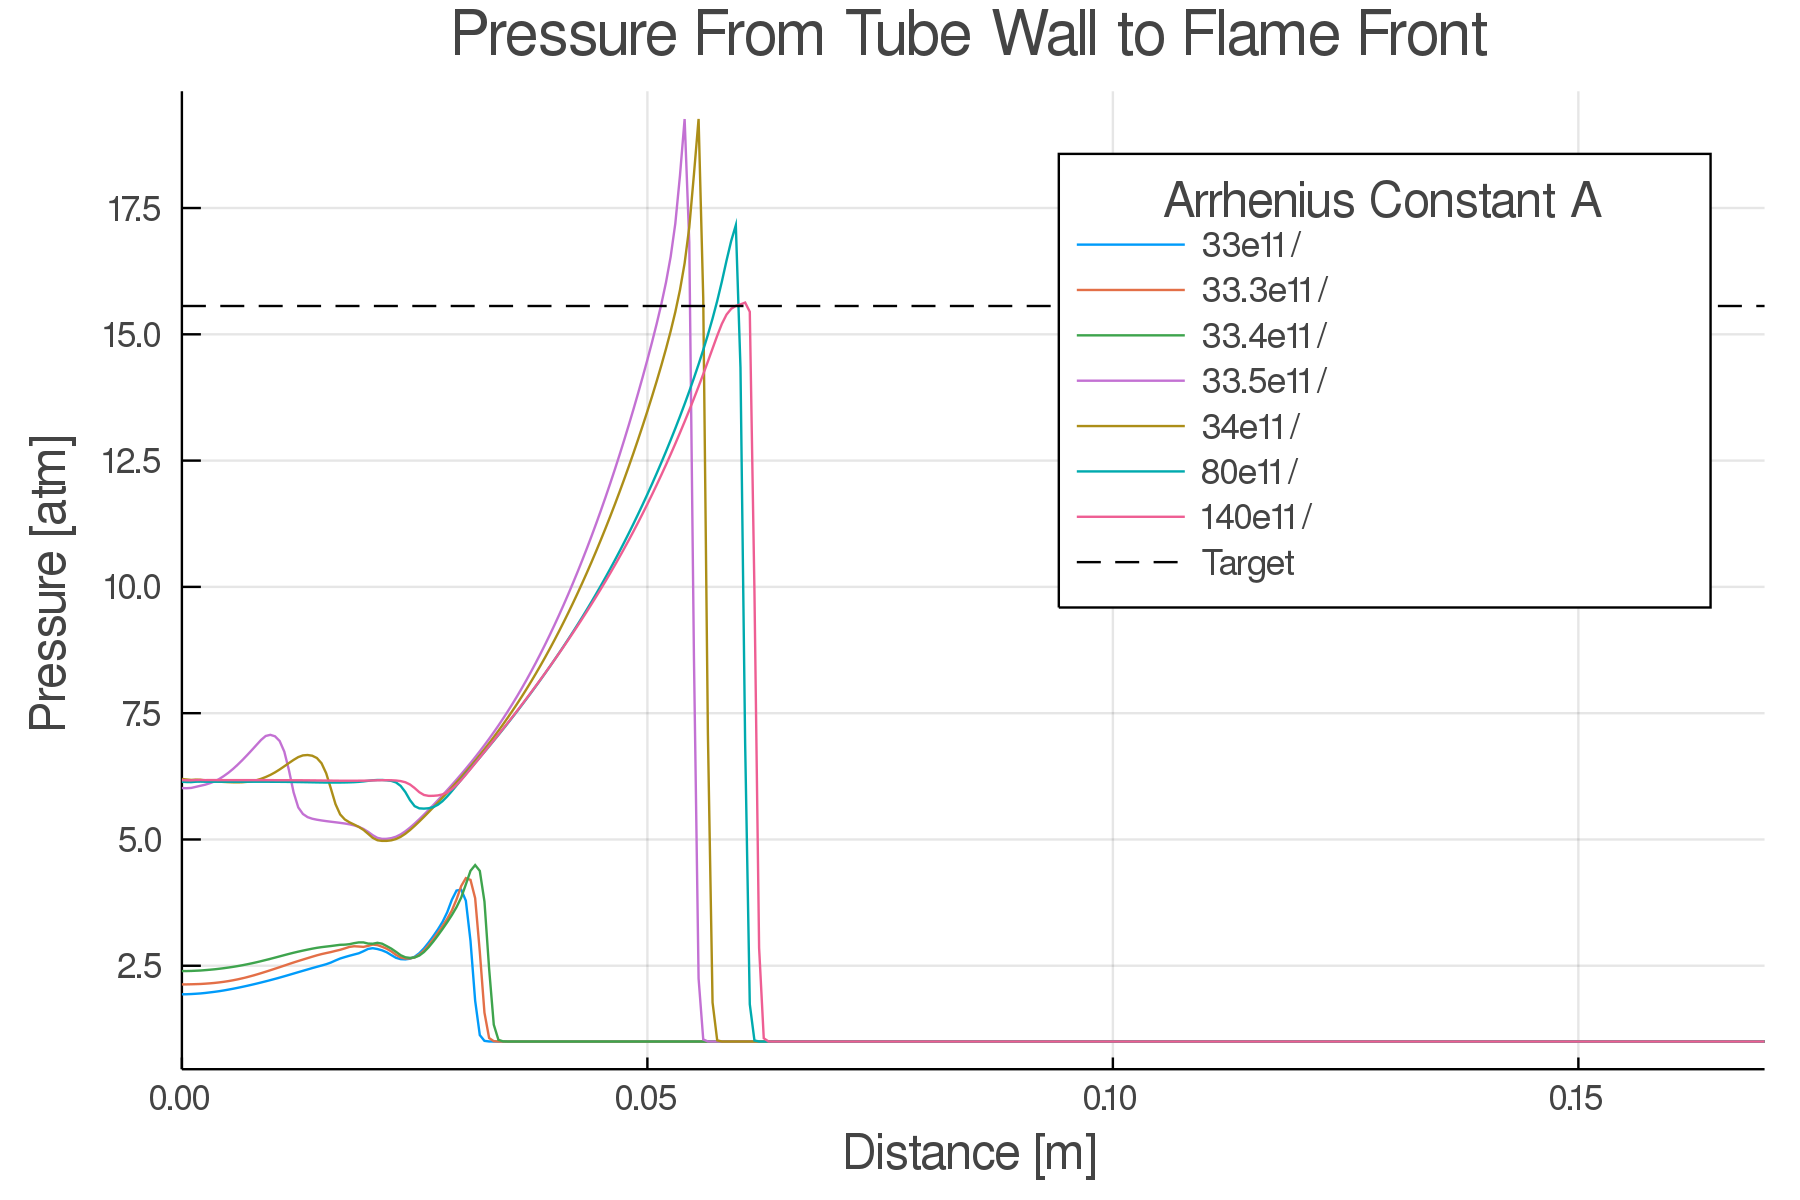
\includegraphics[width=0.85\linewidth]{./figs/Atest_refined/p.png}
\caption{Pressure distribution in detonation tube for refined pre-exponential factor exponent sweep test, filtered from Figure \ref{fig:pjump} and refined from Figure \ref{fig:atestp}}
\label{fig:atestrp}
\end{figure}

\begin{figure}
\centering
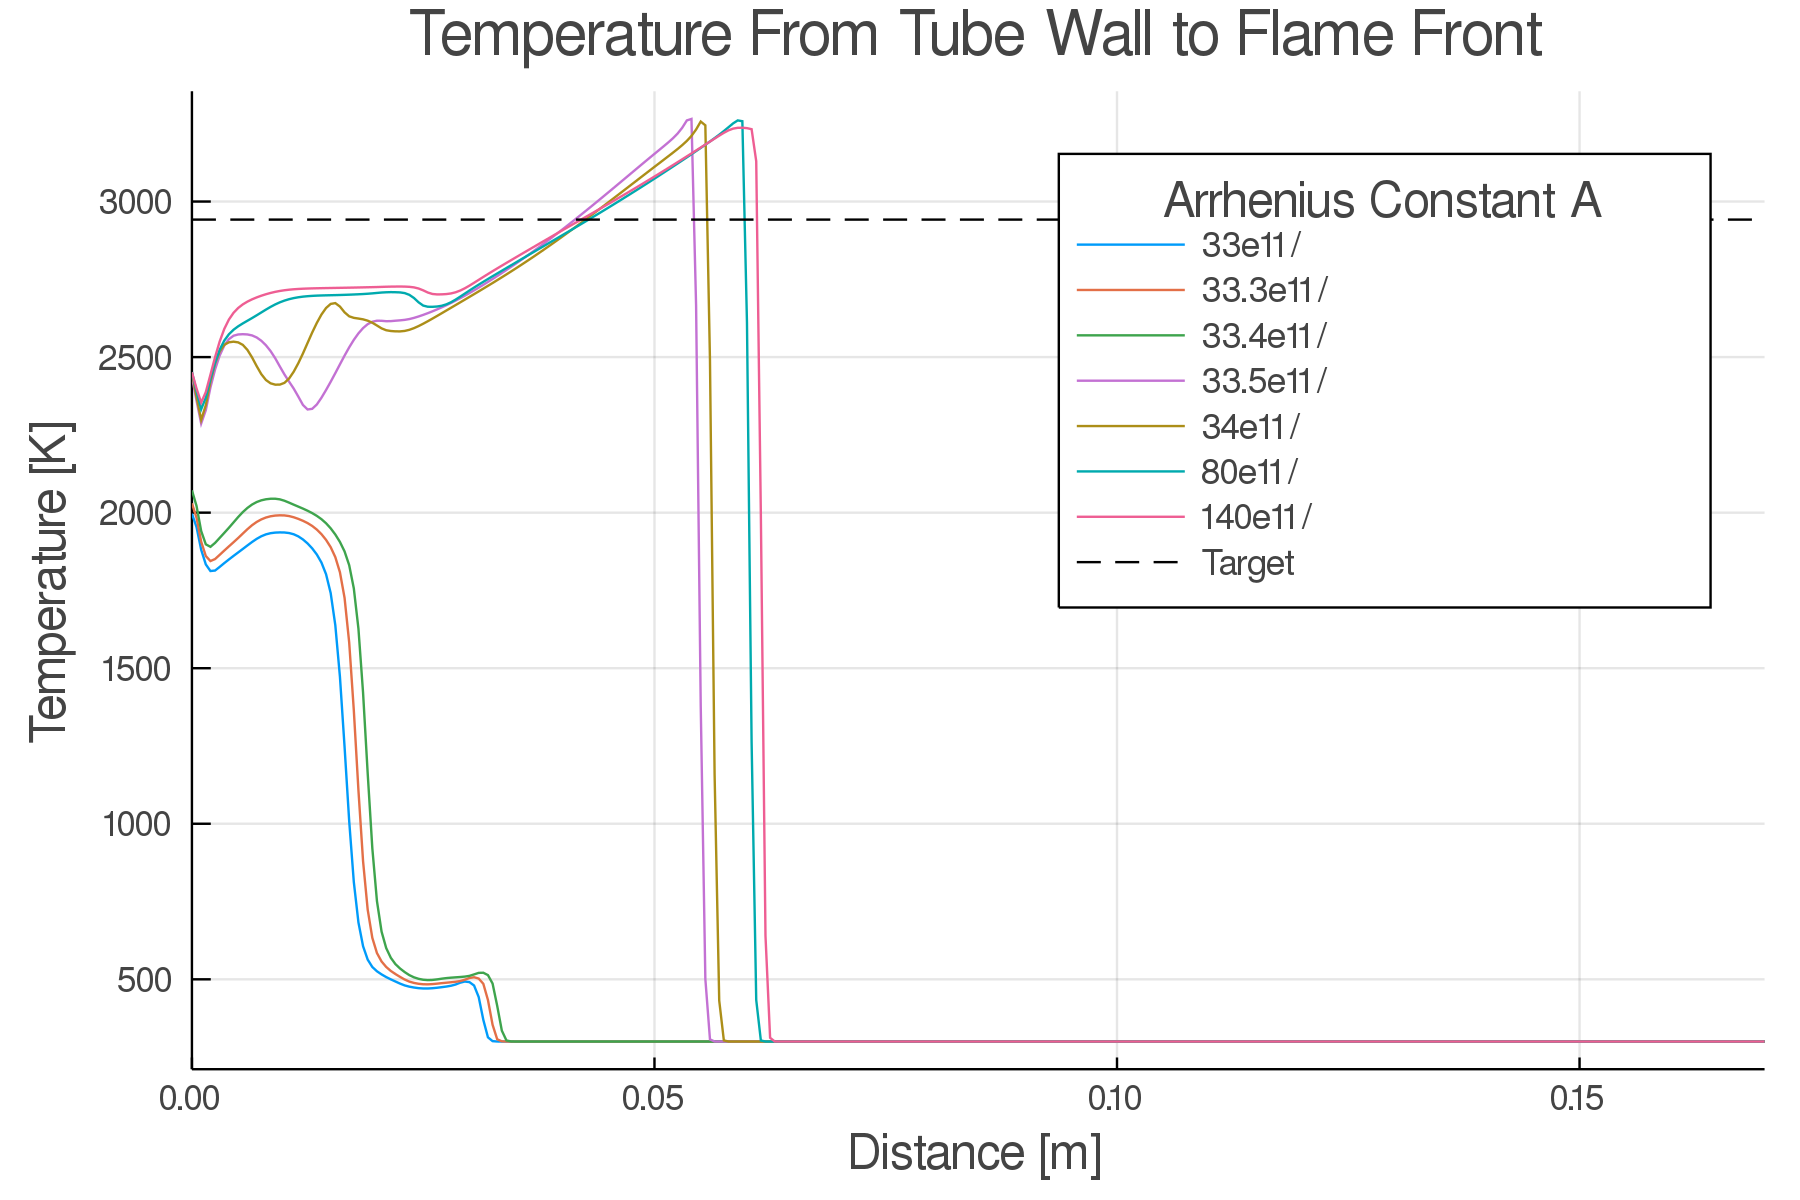
\includegraphics[width=0.85\linewidth]{./figs/Atest_refined/t.png}
\caption{Temperature distribution in detonation tube for refined pre-exponential factor exponent sweep test, refined from Figure \ref{fig:atestt}}
\label{fig:atestrt}
\end{figure}

With these tests, \(10^{13}\) was selected as an appropriate order of magnitude as it not only agreed with the results seen in Towery\cite{towery1}, but also with the value given for a single-step hydrogen-oxygen detonation in other published works\cite{hashemi}. 




\subsection{Time Step Variation}
One of the important tests was to determine how large the time step of the simulation could be taken. In OpenFOAM, one has several options for how the time step should be selected. By default, time steps are fixed, and set within \verb|controlDict|. Setting different values for how large the time step should be will affect the stability and solution of the simulation. Larger time steps will be more unstable, increasing the Courant number and sometimes leading towards the inability for solutions at a time step to converge. If we consider a fluid particle, the faster it moves, the more distance it can cover in a unit of time. If it is moving very quickly, large time steps mean this fluid particle could have traversed very far, leading to uncertainty in the solution. In a more general sense, we consider information and how it progresses throughout the gridded domain. For Courant numbers larger than one, the fluid is moving through more than one grid point per time step, and this is very difficult for the time integrators solving the flow equations to assess accurately. The logical choice would be to always select a very small time step to ensure a more stable and accurate solution. However, with decreased time step intervals comes increased computational cost, as the computer must solve the fluid equations much more often to arrive at a specific point in time. Instead, a smarter approach can be taken, where the time step is allowed to vary based on the Courant number. 

Inside \verb|controlDict| for \verb|rhoReactingCentralFoam|, we can set a maximum for both the typically-used fluid velocity Central Courant number as well as the acoustic (wave speed) Courant number. Each iteration, the solver will check the value of both these Courant numbers, and decrease the time step accordingly if the Courant number maximum is exceeded. In an effort to best determine how large the Courant number and therefore the time step can be, the maximum Courant number was set and swept across for various values. For these tests, a domain size of \( (x,y,z) = (0.5,0.04,0.04) \) meters was used with a 5000-3-3 mesh. This is pseudo-one-dimensional setup. Several maximum Courant (CFL) numbers were swept across, and the results at \(3\times 10^{ - 5}\)s are plotted in Figures \ref{fig:cflp}, \ref{fig:cflt}, and \ref{fig:cflu}. Note that the notation used in the plot omits the decimal point for the maximum CFL number, so \verb|5000_3_3_005| represents a 5000-3-3 mesh with a maximum CFL of 0.05. 

\begin{figure}
    \centering
    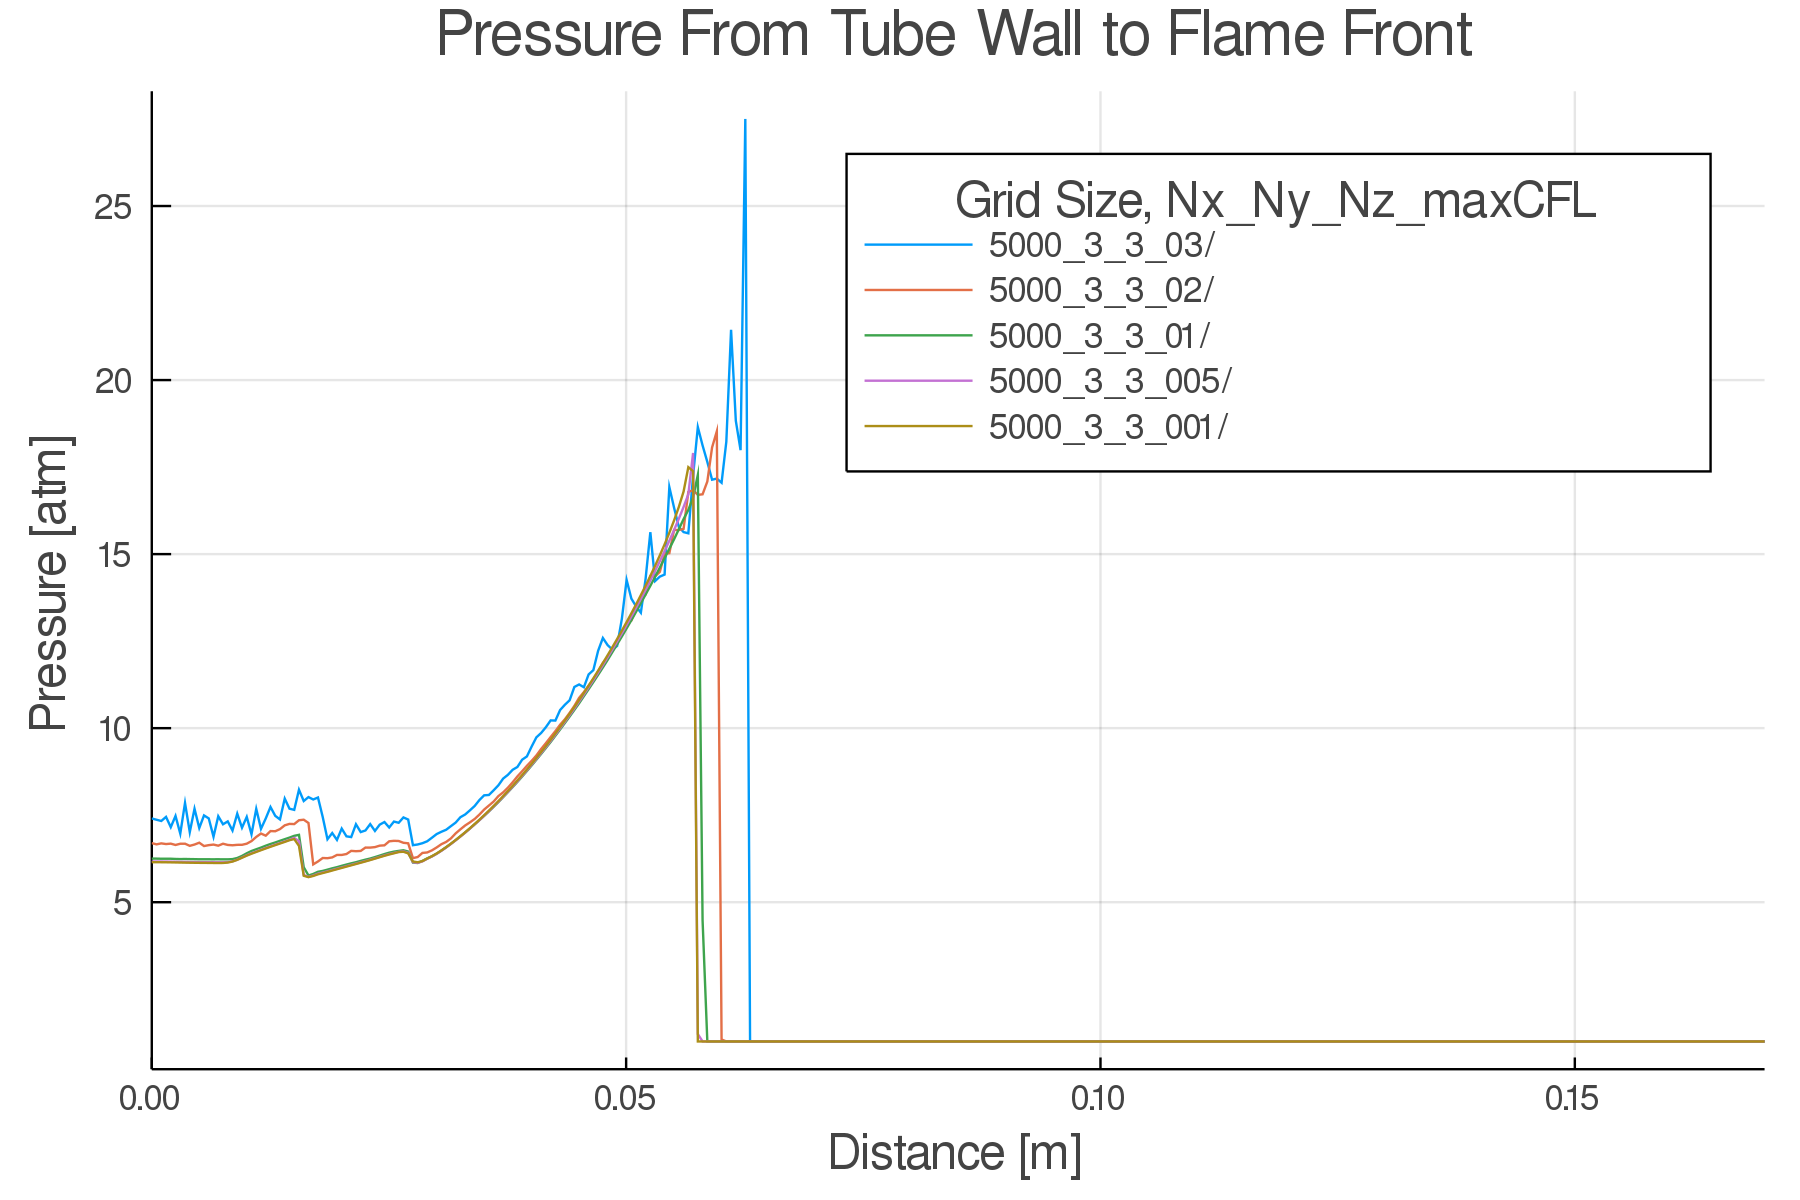
\includegraphics[width=0.85\linewidth]{figs/cfl_test/p.png}
    \caption{Pressure distribution for max CFL sweep}
    \label{fig:cflp}
\end{figure}

\begin{figure}
    \centering
    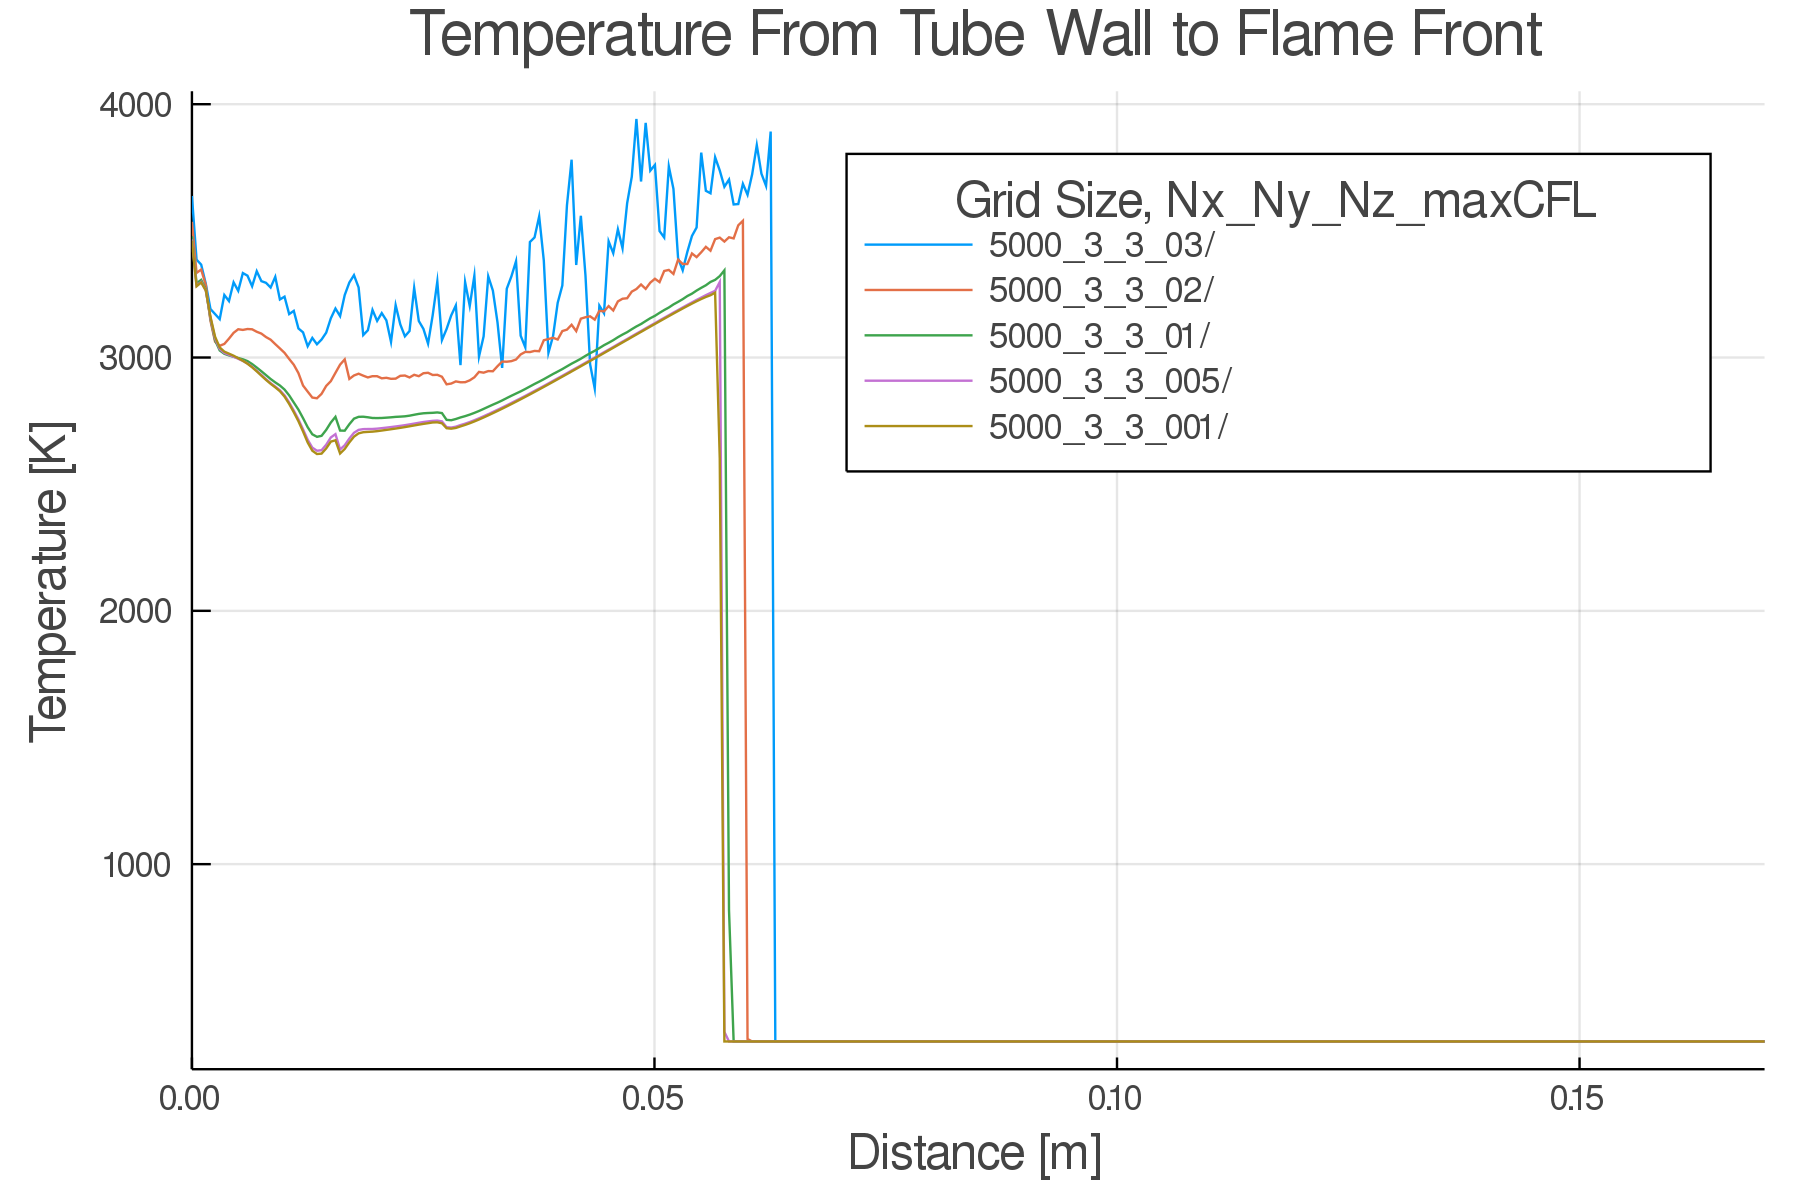
\includegraphics[width=0.85\linewidth]{figs/cfl_test/t.png}
    \caption{Temperature distribution for max CFL sweep}
    \label{fig:cflt}
\end{figure}

\begin{figure}
    \centering
    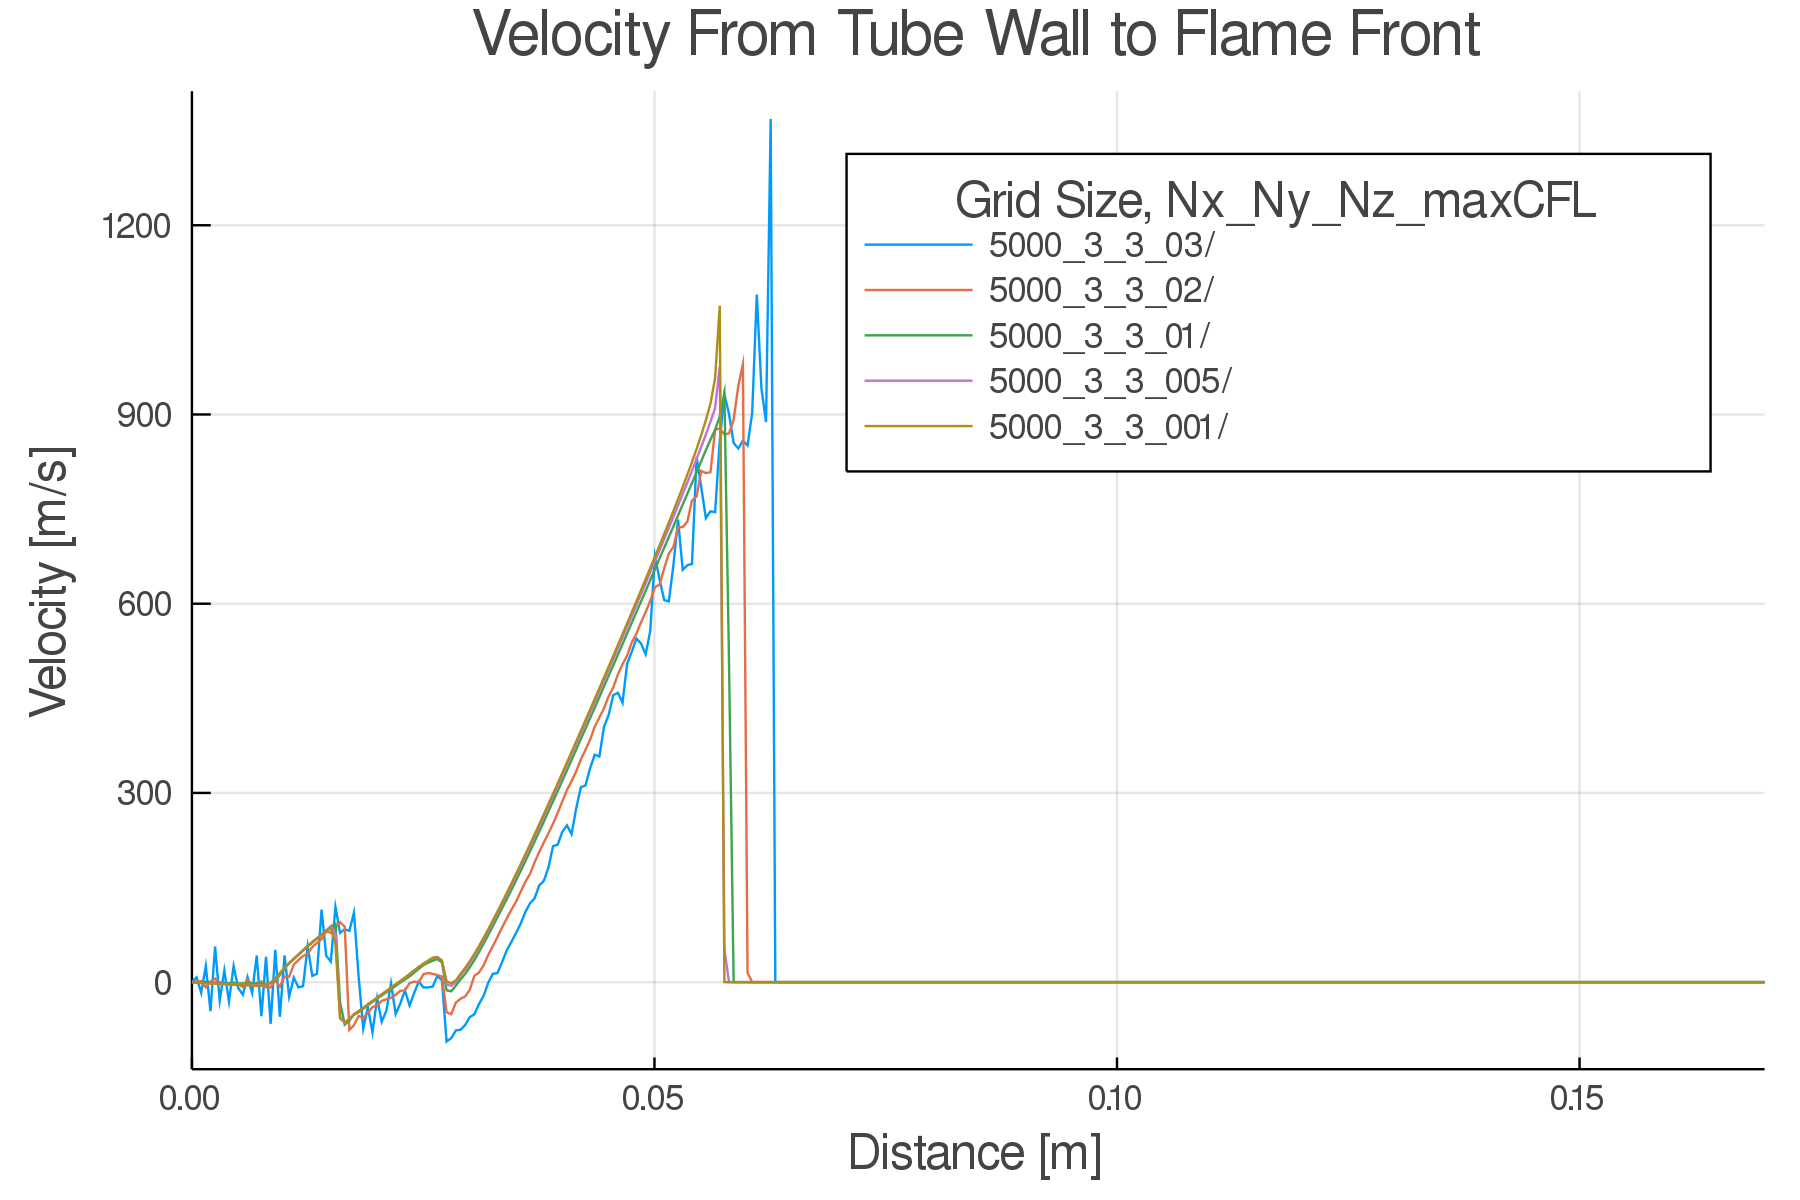
\includegraphics[width=0.85\linewidth]{figs/cfl_test/u.png}
    \caption{Velocity distribution for max CFL sweep}
    \label{fig:cflu}
\end{figure}

From Figures \ref{fig:cflp}, \ref{fig:cflt}, and \ref{fig:cflu}, it is seen that there is decreased noise in the solution as well as convergence as the time step and therefore maximum CFL is decreased. More evident in the temperature plot \ref{fig:cflt}, noise and instability is especially clear in the detonation simulations with maximum CFLs of 0.2 and 0.3. The CFL of 0.1 was decided to be acceptably converged due to a small comparative error, seen in Table \ref{tab:cflerror}. 
\begin{table}[]
\centering
\caption{Max CFL errors compared to CFL = 0.01}
\label{tab:cflerror}
\begin{tabular}{cccc}
Max CFL & Pressure Error (\%) & Temperature Error (\%) & Velocity Error (\%) \\ \hline
0.3 & 57.18 & 19.54 & 27.62 \\ 
0.2 & 5.89 & 8.72 & 8.66 \\
0.1 & 1.28 & 2.71 & 12.92 \\
0.05 & 2.34 & 1.29 & 8.96 \\
0.01 & 0 & 0 & 0 \\
\end{tabular}
\end{table}% 
\noindent Note that while the CFL of 0.2 has a smaller velocity error than the CFL of 0.1, it is a much noisier and unstable solution, so the values themselves have further uncertainty. The selection of a maximum CFL of 0.1  for detonations in OpenFOAM also matches with the work done by Ajaero\cite{ajaero}. 

\subsection{Static Mesh Variation}

\subsection{Adaptive Mesh Refinement and Static Comparisons}

\subsection{Sensitivities, efficiencies of AMR?}